
\documentclass[tikz,border=6pt]{standalone}
\usepackage{amsmath}
\usepackage{tikz}
\usetikzlibrary{angles,quotes}

\begin{document}
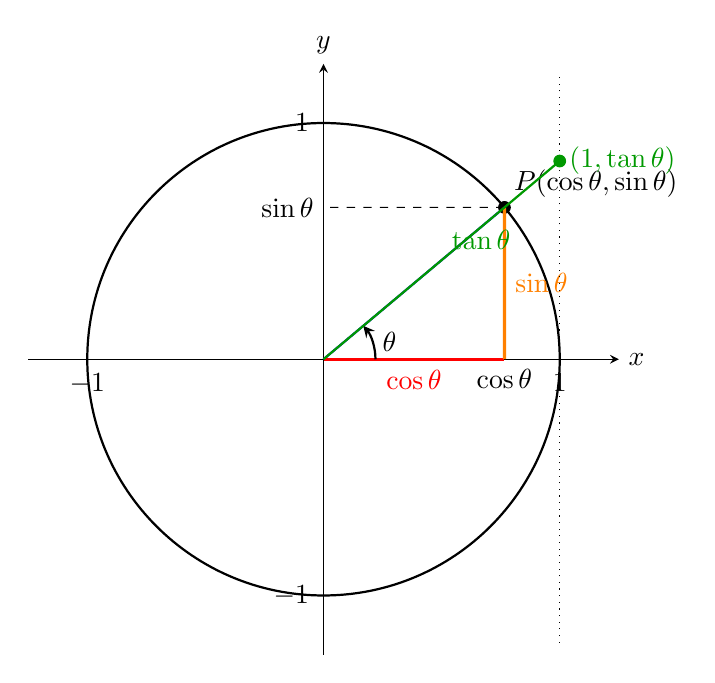
\begin{tikzpicture}[scale=3, >=stealth]

  \def\R{1}
  \def\ang{40} % angle in degrees

  \coordinate (O) at (0,0);
  \coordinate (P) at ({cos(\ang)},{sin(\ang)});

  % axes
  \draw[->] (-1.25,0) -- (1.25,0) node[right] {$x$};
  \draw[->] (0,-1.25) -- (0,1.25) node[above] {$y$};

  % unit circle
  \draw[thick] (O) circle (\R);

  % axis ticks and labels
  \draw (-1,0) -- ++(0,-0.02) node[below] {$-1$};
  \draw (1,0) -- ++(0,-0.02) node[below] {$1$};
  \draw (0,-1) -- ++(-0.02,0) node[left] {$-1$};
  \draw (0,1) -- ++(-0.02,0) node[left] {$1$};

  % radius to point P
  \draw[thick, blue] (O) -- (P);
  \filldraw (P) circle (0.7pt)
    node[above right] {$P(\cos\theta,\sin\theta)$};

  % projections
  \draw[dashed] (P) -- ({cos(\ang)},0)
    node[below] {$\cos\theta$};
  \draw[dashed] (P) -- (0,{sin(\ang)})
    node[left] {$\sin\theta$};

  % colored sine / cosine segments
  \draw[very thick, red]
    (O) -- ({cos(\ang)},0) node[midway, below] {$\cos\theta$};
  \draw[very thick, orange]
    ({cos(\ang)},0) -- (P) node[midway, right] {$\sin\theta$};

  % angle arc
  \draw[->, thick]
    (0.22,0) arc (0:\ang:0.22)
    node[midway, right] {$\theta$};

  % tangent line & intersection
  \draw[dotted] (1,-1.2) -- (1,1.2);
  \coordinate (T) at (1,{tan(\ang)});
  \draw[green!60!black, thick] (O) -- (T)
    node[midway, above right] {$\tan\theta$};
  \filldraw[green!60!black] (T) circle (0.7pt)
    node[right] {$(1,\tan\theta)$};

\end{tikzpicture}
\end{document}
